This chapter will show use cases showing how the simulator can be used.

\section{Use case 1}
	\subsection*{2 Versus 2}
	This first use case will show a battle between 2 teams each having the same regiments.
	The first team is a group of Pirates and the other team is a group of Ninjas. The grid is a $4 \times 4$ map. \\
	Team Pirates are shown here. The regiments are also present in the Ninja team file, but with names starting with Ninja.
\begin{lstlisting}
Regiment PirateArcher
{
	Size = 10;
	Type = Ranged;
	Range = 2;
	Damage = 4;
	Health = 4;
	Movement = 1;
	AttackSpeed = 1;
	RegimentPosition = Position(4,5);
	Behaviour ArcherBehaviour
	{
		Regiment enemy = SearchForEnemies();
		if (enemy.Distance <= Range)
		{
			Attack(enemy);
			if(enemy.Distance < 2)
			{
				MoveAway(enemy);
			}
		}
		else
		{
			MoveTowards(enemy);
		}
	}
}
Regiment PirateWarrior
{
	Size = 10;
	Type = Melee;
	Damage = 8;
	Health = 4;
	Movement = 1;
	AttackSpeed = 1;
	RegimentPosition = Position(2,5);
	Behaviour WarriorBehaviour
	{
		Regiment enemy = SearchForEnemies();
		if (enemy.Distance <= Range)
		{
			Attack(enemy);
		}
		else
		{
			MoveTowards(enemy);
			Attack(enemy);
		}
	}
}
\end{lstlisting}

	\subsection*{Screenshots from use case 1}
		\begin{figure}[H]
			\center
			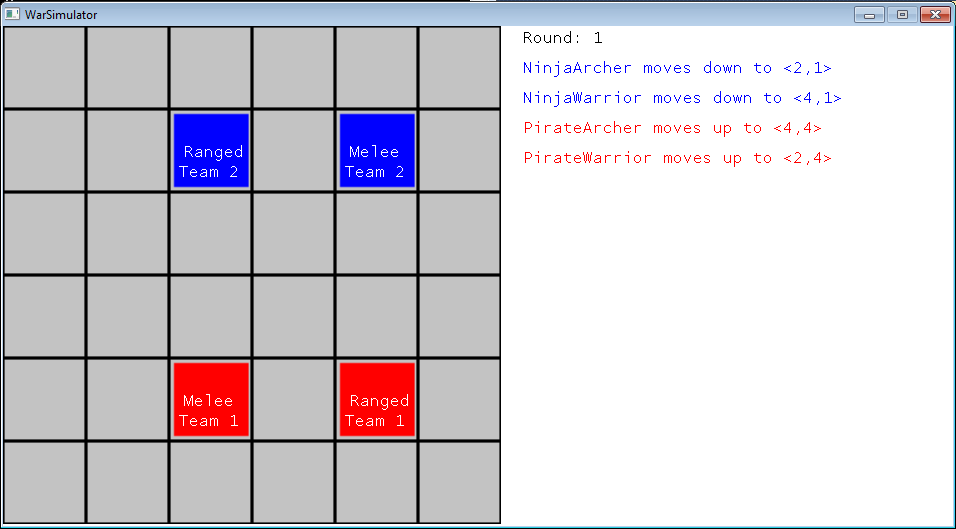
\includegraphics[scale=0.6]{rapport/7/figures/case1-1.png}
			\caption{The battle begins}
		\end{figure}
		\begin{figure}[H]
		\center
			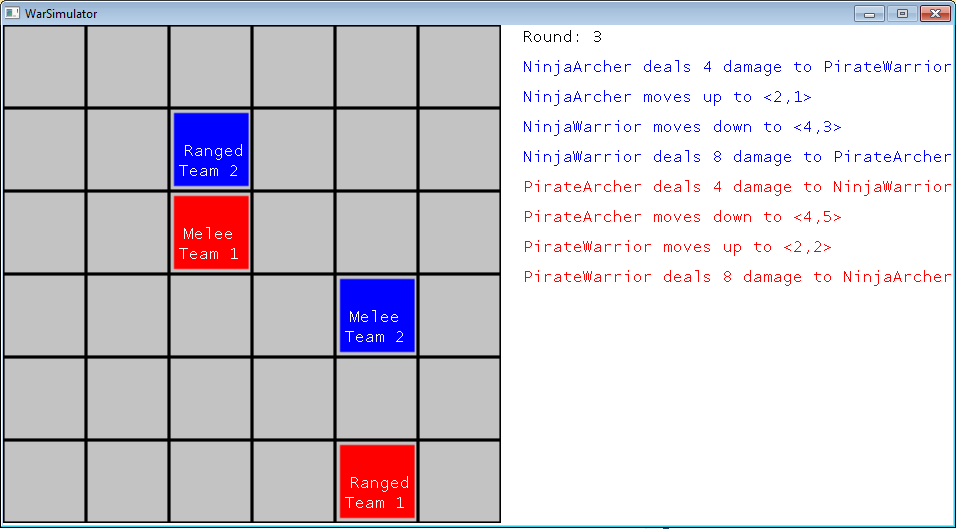
\includegraphics[scale=0.6]{rapport/7/figures/case1-2.png}
			\caption{The Warriors chase the archers}
		\end{figure}
		\begin{figure}[H]
		\center
			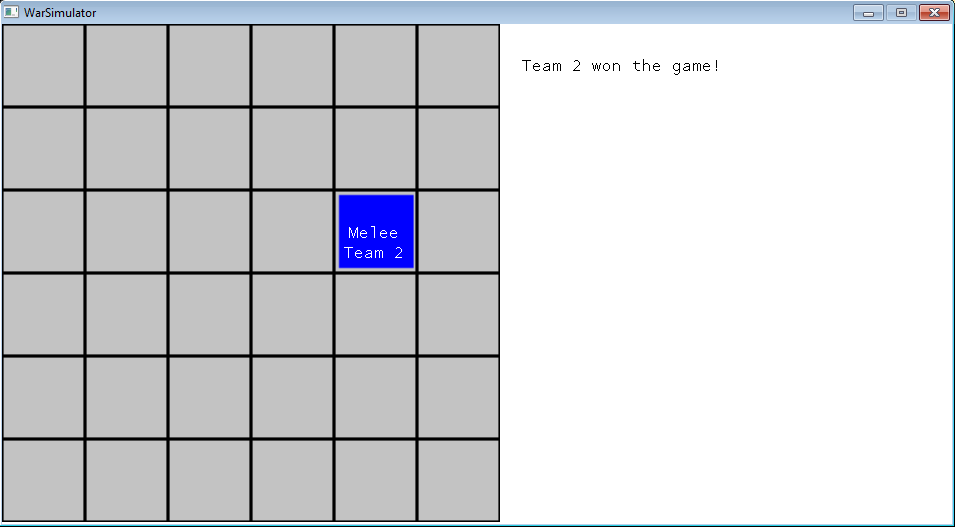
\includegraphics[scale=0.6]{rapport/7/figures/case1-3.png}
			\caption{Team 2 won!}
		\end{figure}
		
\section{Use case 2}
	\subsection*{Big battle}
	This use case will show a big battle between 4 teams. This scenario also showcases how the grid will scale when the 
	grid size is increased. In this battle the grid size is $10 \times 10$
	
	\subsection*{Screenshots from use case 2}
		\begin{figure}[H]
			\center
			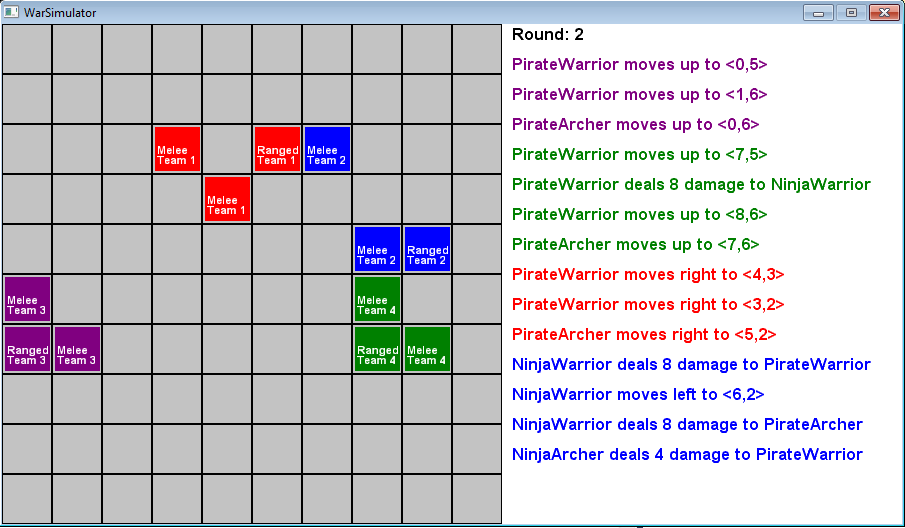
\includegraphics[scale=0.6]{rapport/7/figures/case2-1.png}
			\caption{The battle begins}
		\end{figure}
		\begin{figure}[H]
		\center
			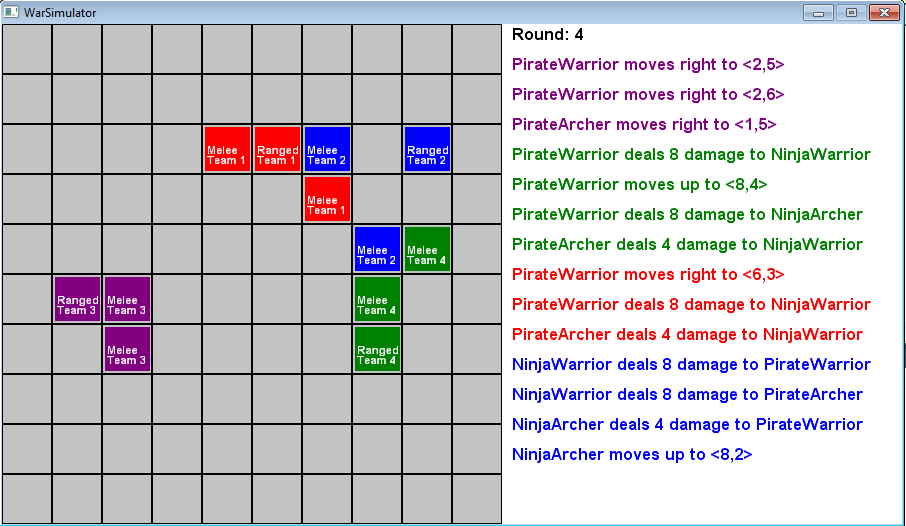
\includegraphics[scale=0.6]{rapport/7/figures/case2-2.png}
			\caption{Team 3 is being passive}
		\end{figure}
		\begin{figure}[H]
		\center
			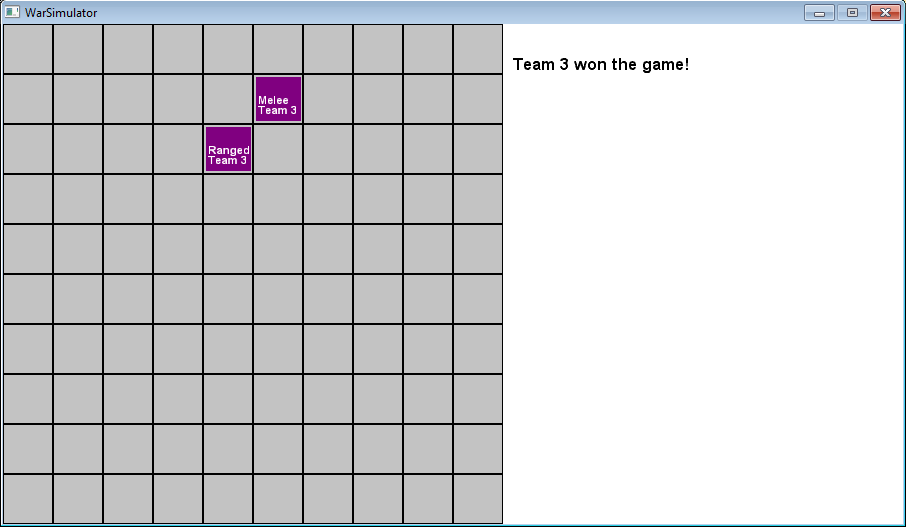
\includegraphics[scale=0.6]{rapport/7/figures/case2-3.png}
			\caption{Team 3 won!}
		\end{figure}
	
\section{Usecase 3}
In this usecase, we will explore the scripts of an experienced scripter versus an inexperienced scripter. The experienced scripter wrote Team 1 and the inexperienced scripter wrote Team2. Team 2 consist of one slow, but dangerous melee regiment called KlamBymilits. The scriptwriter behind team 2 in convinced this regiments high damage will make it possible for him to take out both of the opponents regiments. The regiments behaviour is extremely simple - attack any nearby enemies, and if no enemies are within range, start moving towards the enemy. The scripter behind team 1 has two regiment of archers with considerably less health. These regiments are required to use their speed and positions to conquer their enemy. The archers will spawn on each side of the enemy regiment. The behaviour of the archer regiments is designed to take advantage of the slow movement and simple tactic of the enemy. When the distance between one archer regiment and the enemy, is less than the distance between the enemy and the other archer, the archer regiment moves away from the enemy regiment. If the distance is greater, than the distance between the enemy and the friendly archer regiment, the archer regiment attacks and moves towards the enemy. The result is quite spectacular - the archers successfully kite the enemy regiment in circles, and win without taking any damage.
\begin{lstlisting}
Team Team1

Regiment Archers1
{
	Size = 50;
	Range = 10;
	Damage = 10;
	Movement = 5;
	AttackSpeed = 2;
	Health = 20;
	Type = Ranged;
	RegimentPosition = Position(5,5);
Behaviour HitnRun
{
	Regiment enemy = SearchForEnemies();
	Regiment friend = SearchForFriends();
	if(enemy.Distance < (friend.Distance-enemy.Distance))
	{
		MoveAway(enemy);
		MoveAway(enemy);
	}
	else
	{
		if(enemy.Distance < Range)
		{
			Attack(enemy);
		}
		else
		{
			MoveTowards(enemy);
			MoveTowards(enemy);
		}
	}
	Attack(enemy);
}
}


Regiment Archers2
{
	Size = 50;
	Range = 10;
	Damage = 10;
	Movement = 5;
	AttackSpeed = 2;
	Health = 20;
	Type = Ranged;
	RegimentPosition = Position(15,15);
Behaviour HitnRun
{
	Regiment enemy = SearchForEnemies();
	Regiment friend = SearchForFriends();
	if(enemy.Distance < (friend.Distance-enemy.Distance))
	{
		MoveAway(enemy);
		MoveAway(enemy);
	}
	else
	{
		if(enemy.Distance < Range)
		{
			Attack(enemy);
		}
		else
		{
			MoveTowards(enemy);
			MoveTowards(enemy);
			MoveTowards(enemy);
		}
	}
	Attack(enemy);
}

}
\end{lstlisting}

\begin{lstlisting}
Team Team2

Regiment KlamBymilits
{
	Size = 20;
	Damage = 20;
	Type = Melee;
	Health = 50;
	Movement = 2;
	AttackSpeed = 1;
	RegimentPosition = Position(10,10);
Behaviour StupidBehaviour
{
	Regiment enemy = SearchForEnemies();
	if (enemy.Distance > 1)
	{
		MoveTowards(enemy);
	}
	else
	{
		Attack(enemy);
	}
}
}
\end{lstlisting}

	\subsection*{Screenshots from use case 3}
		\begin{figure}[H]
			\center
			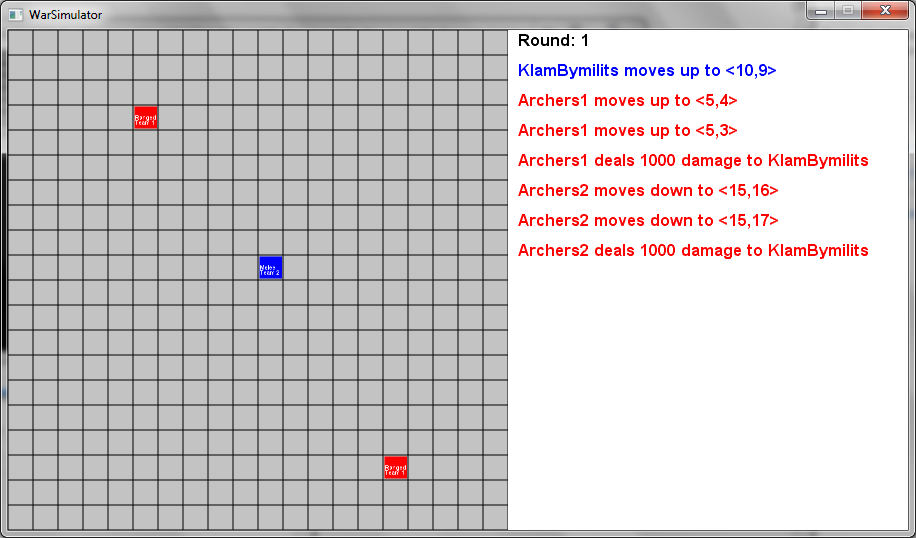
\includegraphics[scale=0.6]{rapport/7/figures/case3-1.png}
			\caption{The battle begins.}
		\end{figure}
		\begin{figure}[H]
		\center
			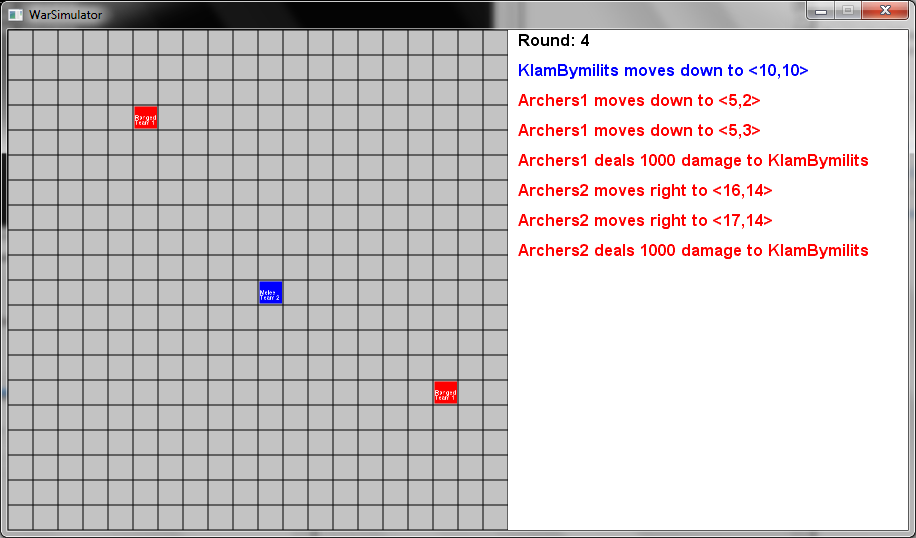
\includegraphics[scale=0.6]{rapport/7/figures/case3-2.png}
			\caption{The blue team is hesitant to attack either of the red archers.}
		\end{figure}
		\begin{figure}[H]
		\center
			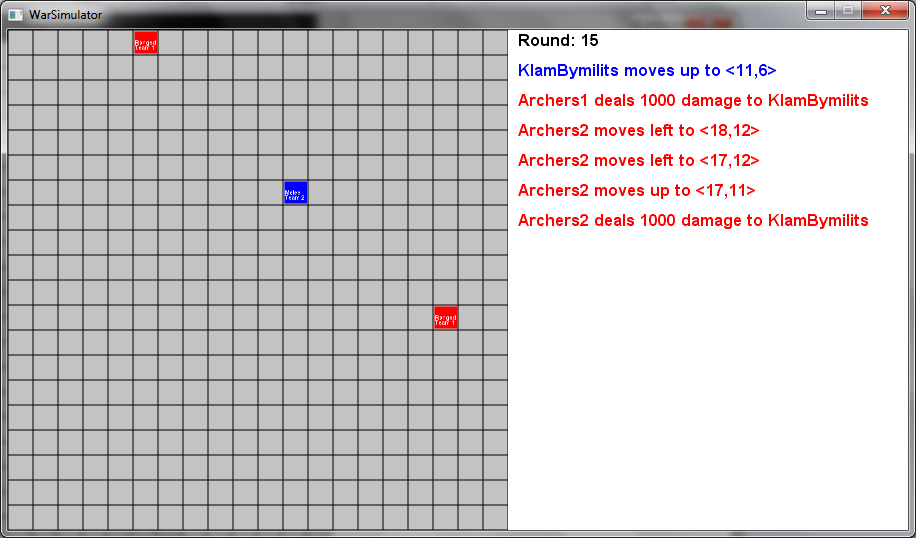
\includegraphics[scale=0.6]{rapport/7/figures/case3-3.png}
			\caption{Even after 15 rounds, the blue team is only a little better off.}
		\end{figure}